%!TEX program = xelatex
%!TEX builder = latexmk
% or can be latexmk texify
%!TEX option = --output-driver="xdvipdfmx -V7"
% -shell-escape -8bit % For minted package
%!TEX root = ...
\documentclass[11pt,a4paper,twocolumn,fleqn]{article} % titlepage表示标题单独页
\usepackage{ctex} % ctex套用英文标题格式 (建议在英文论文混排中文时使用) ,
% ctexcap套用中文格式 (等同于\documentclass{ctexart}) 
% \renewcommand{\figurename}{图}
% \renewcommand{\tablename}{表}
% \renewcommand{\contentsname}{目录}
% \renewcommand\refname{参考文献}
% \renewcommand{\thefigure}{\chinese{figure}} % 将图片计数改为汉字数字
% \renewcommand{\thetable}{\chinese{table}} % 将表格计数改为汉字数字
\usepackage[top=0.75in,bottom=0.75in,left=0.75in,right=0.75in]{geometry} % 页边距设置
% \usepackage{multicol}页面内多行包
\usepackage[CJKbookmarks]{hyperref} % 给pdf文档添加互动式链接和书签
% \userpackage{wrapfig} % 图文绕排
% \usepackage{xeCJK} % to get my Chinese name
% \setCJKmainfont{SimSun}
% \usepackage[parfill]{parskip} % 增加段间行距
\usepackage{amsmath,amssymb,esint} % 数学公式类宏包;最末为积分符号拓展
\allowdisplaybreaks[0]% 允许多行公式间换页, 用//*表示不允许换页
% \numberwithin{equation}{section} % 公式编号包含章节
\usepackage{bm} % 加粗 (用于vector) 
% \usepackage{mathrsfs} % mathscr font
% \usepackage{textcomp} % 符号包, 不能用于数学模式, 建议不要和SIunits混用
% \usepackage[squaren]{SIunits} % 科学单位包, 可以用于数学模式
% (为了统一不要和textcomp混用) , squaren选项消除和amssymb的冲突
\usepackage{siunitx} % 淘汰掉上面这个宏包吧, 现在用的是
% \num{123}, \si{kg.m/s^2}, 
% \si{\electronvolt\per\square\clight}, \SI{123}{\micro\metre}
\usepackage{extarrows} % 长箭头, 长等号etc.
\usepackage{graphicx} % 插图宏包
% \usepackage{picinpar} % 图文绕排
\usepackage{array} % 表格宏包
% \usepackage{longtable} % 长表格宏包
\usepackage{multirow} % 多行合并的表格宏包
% \usepackage{booktabs} % 表格线宏包
% \usepackage{braket} % 狄拉克符号
\usepackage{xcolor}

% \usepackage[basic,box,gate,oldgate,ic,optics,physics]{circ} % 电路图宏包
% \usepackage[normalem]{ulem} % 下划线, 删除线等宏包, 参数表示不修改\emph{}格式
% \usepackage{mychemistry} % 化学宏包, 包含mhchem和chemfig
% \usepackage[version=3]{mhchem} % 化学宏包, 包含mhchem和chemfig
% \usepackage[symbol]{footmisc} % 脚注拓展, 选项表示用符号做脚注记号
\usepackage{listings} % 代码段宏包
\lstset{numbers=left,frame=shadowbox,%
basicstyle=\ttfamily, commentstyle=\fontseries{lc}\selectfont\itshape, %
columns=fullflexible, breaklines=true, escapeinside={(*@}{@*)}}
% \usepackage{minted} % 具有 Python 支持的代码宏包

% \renewcommand*{\vec}[1]{\bm{#1}} % 矢量的格式, 这里是加粗
\newcommand{\dif}{\,\mathrm d}
\newcommand\mi{\mathrm{i}}
\newcommand\e{\mathrm{e}} % 定义数学模式中常用的正体字符
\newcommand\nf{\ensuremath{\mathrm{n.f.}}}
\newcommand\nnf{\ensuremath{\mathrm{n.n.f.}}}
\renewcommand{\emptyset}{\varnothing}
\DeclareMathOperator{\dom}{dom}
\DeclareMathOperator{\ran}{ran}
\DeclareMathOperator{\fld}{fld}
% \bibliographystyle{unsrt}
\begin{document}
\title{数理逻辑课程整理}
\author{吕铭 Lyu Ming}
\maketitle
\tableofcontents
\section{命题逻辑} % (fold)
\label{sec:propositional_logic}
\subsection{命题逻辑的基本定义} % (fold)
\label{sub:def}
\begin{enumerate}
	\item 术语: 简单命题, 复合命题, 命题变项
	\begin{itemize}
		\item 合式公式 (Wff, 命题): 有限次递归定义
		\item 解释 $I$: 对于命题的各命题变项指定真值
		\item 文字: 命题变项 $P$ 及其否定式 $\lnot P$
		\item 互补对: $P$ 与 $\lnot P$
		\item 合 (析) 取式: 一些文字的合 (析) 取组成的公式
	\end{itemize}
	\item 逻辑联结词: \\
	\begin{centering}
	\begin{tabular}{ccc}
		联结词 & 符号 & 优先级 \\\hline
		否定词 (negation)     & $\lnot$ & 0 \\
		合取词 (conjunction) & $\land$  & 1 \\
		析取词 (disjunction) & $\lor$   & 2 \\
		蕴涵词 (implication) & $\to$    & 3 \\
		双条件词 (biconditional) & $\leftrightarrow$ & 4 \\\hline
		异或 & $\overline\lor$, $\oplus$ \\
		与非 & $\uparrow$ \\
		或非 & $\downarrow$
	\end{tabular}
	\end{centering}
	\item 重言式 (Tautology), 矛盾式, 可满足式 (含重言式)
	\item 代入规则: 一个重言式, 对其中\emph{所有}相同的
	\emph{命题变项} $P$ 都用一合式公式 $X$ 代换, 其结果仍为一重言式. 记作
	$\frac{P}{X}$
\end{enumerate}
\subsection{波兰表达式} % (fold)
\label{sub:polish}
\begin{itemize}
	\item 波兰表达式: 所有符号使用前置式
	\item 逆波兰表达式: 所有符号使用后置式
\end{itemize}
% subsection polish (end)
% subsection def (end)
\subsection{命题逻辑的等值性} % (fold)
\label{sub:logic_calculation}
\begin{enumerate}
	\item 等值: 若在其中的任一解释下, 公式 $A$ 和 $B$ 的真值都相同. 
	记作 $A = B$ 或 $A\Leftrightarrow B$
	\begin{itemize}
		\item 充要条件: $A\leftrightarrow B$ 是重言式
	\end{itemize}
	\item 逆命题, 否命题, 逆否命题
	\begin{itemize}
		\item 一个命题与它的逆否命题等值
		\item 一个命题的逆命题与它的否命题等值
	\end{itemize}
\end{enumerate}
\subsection{等值公式} % (fold)
\label{sub:logic_equ}
\begin{enumerate}
	\item 基本等值公式 (命题定律):
	\begin{itemize}
		\item 双重否定率: $\lnot\lnot P = P$
		\item 结合律, 交换律: $\lor, \land, \leftrightarrow$
		\item 分配率: $\lor$ 对 $\land$; $\land$ 对 $\lor$, $\to$ 对 $\to$
		\item 等幂律 (恒等率)\\
		$P\lor P = P\land P = P$ \\
		$P\to P = P\leftrightarrow P = T$
		\item 吸收率\\
		$P\lor (P\land Q) = P$ \\
		$P\land (P\lor Q) = P$
		\item 摩根率\\
		$\lnot(P\lor Q) = \lnot P\land \lnot Q$ \\
		$\lnot(P\land Q) = \lnot P\lor \lnot Q$ \\
		$\lnot(P\to Q) = P\land \lnot Q$ \\
		$\lnot(P\leftrightarrow Q) = \lnot P\leftrightarrow Q 
		= P\leftrightarrow\lnot Q = (\lnot P\land Q)\lor(P\land\lnot Q)$
		\item 同一律\\
		$P\lor F = P\land T = T\to P = T\leftrightarrow P = P$ \\
		$P\to F = F\leftrightarrow P = \lnot P$
		\item 零率\\
		$P\lor T = T;\quad P\land F = F$ \\
		$P\to T = T;\quad F\leftrightarrow P = T$
		\item 补余率\\
		$P\lor\lnot P = T;\quad P\land\lnot P = F$ \\
		$P\to\lnot P = \lnot P;\quad \lnot P\to P = P;\quad 
		P\leftrightarrow \lnot P = F$
	\end{itemize}
	\item 其他常用公式\\
	$P \to Q = \lnot P \lor Q$\\
	$P\leftrightarrow Q = (P\to Q)\land (Q\to P)$ \\
	$P\leftrightarrow Q = (P\land Q)\lor (\lnot P\land \lnot Q)$ \\
	$P\leftrightarrow Q = (\lnot P\lor Q)\land (P\lor \lnot Q)$ \\
	$P\to(Q\to R) = (P\land Q)\to R$ \\
	$P\to(Q\to R) = Q\to(P\to R)$ \\
	$(P\to R)\land (Q\to R) = (P\lor Q)\to R$
\end{enumerate}
% subsection logic_equ (end)
\subsection{置换规则} % (fold)
\label{sub:sub_rule}
\begin{itemize}
	\item 子公式: $X$ 是合式公式A的一部分, 且 $X$ 本身也是一个合式公式
	\item 置换: 设$X$为公式 $A$的子公式, 用与$X$等值的公式$Y$ 将$A$中的$X$ 代替
	\item 置换规则: 置换前后公式等值
\end{itemize}
% subsection sub_rule (end)
\subsection{命题公式与真值表} % (fold)
\label{sub:equ_and_bool}
如何从真值表获得逻辑表达式
\begin{itemize}
	\item 从 $T$ 来列写, 用 $\lor$ 连接\\
	$(\bullet\land\bullet)\lor(\bullet\land\bullet)\lor(\bullet\land\bullet)$
	\item 从 $F$ 来列写, 用 $\land$ 连接\\
	$(\bullet\lor\bullet)\land(\bullet\lor\bullet)\land(\bullet\lor\bullet)$
\end{itemize}
% subsection equ_and_bool (end)
\subsection{联结词的完备性} % (fold)
\label{sub:comple}
\begin{enumerate}
	\item 真值函项: 所有合式公式关于等值性的等价类
	\item 联结词的完备集: 设 $C$ 是一个联结词的集合, 如果任何 $n$ 元 ($ n\ge 1$)
	真值函项都可以由仅含 $C$ 中的联结词构成的公式表示, 
	则称 $C$ 是完备的联结词集合, 或说 $C$ 是联结词的完备集
	\item $\{\lnot, \lor, \land\}, 
	\{\lnot, \land\}, 
	\{\lnot, \lor\}, 
	\{\lnot, \to\}, 
	\{\uparrow\}, \{\downarrow\}$ 是联结词完备集
\end{enumerate}
% subsection comple (end)
\subsection{对偶式} % (fold)
\label{sub:duality}
对于仅使用联结词 $\lnot, \lor, \land$ 的命题公式, 
\begin{enumerate}
	\item $A$ 作替换 $(\lor, \land, T, F) \to (\land, \lor, F, T)$ 得 $A^*$, 
	$A$ 和 $A^*$ 互为对偶式
	\item 对于 $A = A(P_1, \cdots, P_n)$, 记 
	$A^- = A(\lnot P_1, \cdots, \lnot P_n)$
	\item $\lnot(A^*) = (\lnot A)^*$, $\lnot(A^-) = (\lnot A)^-$
	\item $(A^*)^* = A$, $(A^-)^- = A$
	\item $\lnot A = A^{*-}$ (本质是摩根率)
	\item $A = B$ 则 $A^* = B^*$
	\item $A\to B$ 永真则 $B^*\to A^*$ 永真
	\item $A$ 与 $A^-$; $\lnot A$ 与 $A^*$ 同永真, 同可满足
\end{enumerate}
% subsection duality (end)
\subsection{范式} % (fold)
\label{sub:normal_form}
\begin{enumerate}
	\item 析取范式: 形如 $A_1\lor A_2 \lor \cdots \lor A_n$, 其中 $A_i$ 是合取式
	\item 合取范式: 形如 $A_1\land A_2 \land \cdots \land A_n$, 其中 $A_i$ 是析取式
	\item 范式定理: 任何一命题公式都存在与之等值的合取范式和析取范式
	\item 极小项: $n$ 个命题变项 $P_i$ 组成 $Q_1\land \cdots \land Q_n$ 其中
	$Q_i = P_i$ 或 $\lnot P_i$, 记为 $m_k$ ($0\le k \le 2^n - 1$)
	\begin{itemize}
		\item 每个极小项仅在一个解释下为真
		\item 极小项两两不等值, 且 $m_i\land m_j = F$ $(i\neq j)$
		\item $\bigvee_k m_k = T$
	\end{itemize}
	\item 极大项: $n$ 个命题变项 $P_i$ 组成 $Q_1\lor \cdots \lor Q_n$ 其中
	$Q_i = P_i$ 或 $\lnot P_i$, 记为 $M_k$ ($0\le k \le 2^n - 1$)
	\begin{itemize}
		\item 每个极大项仅在一个解释下为假
		\item 极小项两两不等值, 且 $m_i\lor m_j = T$ $(i\neq j)$
		\item $\bigwedge_k m_k = F$
	\end{itemize}
	\item 主析 (合) 取范式: 仅由极小 (大) 项的析 (合) 取构成的
	析 (合) 取范式称为主析 (合) 取范式
	\item 主析 (合) 取范式定理: 任一含有 $n$ 个命题变项的公式, 
	都存在\emph{唯一}的与之等值的且恰仅含这 $n$ 个命题变项的主析 (合) 取范式
	\item 主范式的转换: 对于各项取极大 (小) 项全集的补集并取非.
	\item 空公式: 
	\begin{itemize}
		\item 永真式的主合取范式为空公式
		\item 矛盾式的主析取范式为空公式
	\end{itemize}
\end{enumerate}
% subsection normal_form (end)
\subsection{推理形式} % (fold)
\label{sub:reasoning}
以符号 (合式公式) 表示的推理关系. 正确的推理形式要求前提真则结论必真. 
\begin{itemize}
	\item 重言蕴含 $\Rightarrow$: 前提 $\Rightarrow$ 结论, 表示公式间的真值关系
	\item $A\Rightarrow B$ 的充要条件是 $A\to B$ 是永真式 / 
	$A\land \lnot B$ 是矛盾式
	\item 基本推理公式
	\begin{enumerate}
		\item $P\land Q \Rightarrow P$ \label{p_and_q}
		\item $\lnot(P\to Q) \Rightarrow P$: \ref{p_and_q} 的推论 \label{notto}
		\item $\lnot (P\to Q) \Rightarrow \lnot Q$: \ref{p_and_q} 的推论
				\label{nottoq}
		\item $P\Rightarrow P\lor Q$
		\item $\lnot P \Rightarrow P\to Q$ \ref{notto} 的逆否
		\item $Q\Rightarrow P\to Q$ \ref{nottoq} 的逆否
		\item $\lnot P \land (P \lor Q) \Rightarrow Q$ \label{notpandp}
		\item $P\land (P\to Q) \Rightarrow Q$: 假言推理, 分离规则, 
				\ref{notpandp} 的变形
		\item $\lnot Q \land (P\to Q) \Rightarrow \lnot P$ \ref{notpandp} 的变形
		\item $(P\to Q)\land (Q\to R) \Rightarrow P\to R$: 三段论
		\item $(Q\to R) \Rightarrow ((P\lor Q) \to (P\lor R))$
		\item $(Q\to R) \Rightarrow ((P\to Q) \to (P\to R))$
		\item ......
	\end{enumerate}
\end{itemize}
% subsection reasoning (end)
\subsection{推理演算} % (fold)
\label{sub:reasoning_calculation}
应用如下规则证明推理形式
\begin{enumerate}
	\item 前提引入规则: 推理过程中可随时引入前提
	\item 结论引入规则: 中间结论可作为后续推理的前提
	\item 代入规则: 仅限于重言式中的命题变项
	\item 置换规则: 利用等值公式对部分公式进行置换
	\item 分离规则: 由 $A$ 及 $A\to B$ 成立,, 可将 $B$ 分离出来
	\item 条件证明规则: $A_1\land A_2 \Rightarrow B$ 与 
	$A_1 \Rightarrow A_2\to B$ 等价
\end{enumerate}
% subsection reasoning_calculation (end)
\subsection{归结法} % (fold)
\label{sub:resolution}
仅有一条归结推理规则的机械推理法, 基于 $A\Rightarrow$ 成立等价于
$A\land \lnot B$ 是矛盾式. 具体步骤:
\begin{enumerate}
	\item $A\land \lnot B$ 出发
	\item 建立子句集 $S$: 取\emph{合取范式} $A\land \lnot B = \bigwedge_i C_i$, 
	$S = \{C_i\}$
	\item 对于 $S$ 中的子句作归结 (消去互补对), 归结结果放入 $S$. 重复此步骤
	\item 直至归结出矛盾式
\end{enumerate}
其中归结式定义: $C_1 = L\lor C_1'$, $C_2 = \lnot L \lor C_2'$ 则归结式 
$R(C_1, C_2) = C_1' \lor C_2'$
% subsection resolution (end)
% section logic_calculation (end)
\subsection{命题逻辑的公理化*} % (fold)
\label{sub:axiomatization}
略...
\begin{enumerate}
	\item 公理系统的结构
	\begin{itemize}
		\item 初始符号: 公理系统内允许出现的全体符号的集合
		\item 形成规则: 公理系统内允许出现的合法符号序列的形成方法与规则
		\item 公理: 精选的最基本的重言式, 作为推演其它所有重言式的依据
		\item 变形规则: 公理系统所规定的推理规则
		\item 建立定理: 公理系统所作演算的主要内容, 
		包括所有的重言式和对它们的证明
	\end{itemize}
	\item 具有代表性的命题逻辑的公理系统\\
	\begin{tabular}{c|cc}
	系统名称 & 年代 & 公理总条数* \\\hline
	Russell          & 1910 & 5 (4) \\
	Frege            & 1879 & 6 (3) \\
	Hilbert—Bernays  & 1934 & 15 \\
	王浩算法         & 1959 & 1** \\
	自然演绎系统     &      & 0***
	\end{tabular}\\
	* 括号内是彼此独立的条数; \\
	** 10 条变形规则; \\
	*** 5 条变形规则
	\item 完备性: 是否所有的重言式或所有成立的定理都可由所建立的公理系统推导出来
	\item 可靠性: 非重言式或者不成立的定理是否也可由所建立的公理系统推导出来
	\item 语义完备性, 语义无矛盾性, 命题演算的可判定性
	\item 非标准逻辑: 如多值逻辑, 模态逻辑
\end{enumerate}
% subsection axiomatization (end)
% section propositional_logic (end)
\section{谓词逻辑} % (fold)
\label{sec:predicate_logic}
\begin{enumerate}
	\item 个体词: 个体词是指所研究对象中可以独立存在的具体的或抽象的客体. 
	\begin{itemize}
		\item 个体常项$a,b,c,\cdots$
		\item 个体变项 $x, y, z, \cdots$
		\item 个体域/论域 $D$
	\end{itemize}
	\item 谓词: 用来刻划个体词的性质或多个个体词间关系的词. 
	又可看作是由给定的个体域到集合 $\{T, F\}$ 上的一个映射, $P, Q, R, \cdots$
	\begin{itemize}
		\item 谓词常项, 谓词变项
		\item 一元谓词 $P(x)$, 多元谓词 $P(x, y, \cdots)$
		\item 命题逻辑中为一个命题是没有个体变项的零元谓词. 
		谓词逻辑符号中命题变项 $p, q, r, \cdots$
	\end{itemize}
	\item 函数: 某一个体域到另一个体域的映射. 谓词逻辑中的函数一般不单独使用, 
	而是嵌入在谓词中. $P(f(x), g(x))$
	\item 量词: 表示个体常项或变项之间数量关系的词
	\begin{itemize}
		\item 全称量词(Universal quantifier) $\forall$ 
		\item 存在量词(xistential quantifier) $\exists$ 
		\item 量词的辖域: 量词所约束的范围称
		\item 约束出现: $(\forall x)$ 和 $(\exists x)$ 辖域中, $x$ 的所有出现
		\item 约束变元: 所有约束出现的变元
		\item 自由变元: 不是约束出现的其它变元
	\end{itemize}
	\item 一阶谓词逻辑: 在所讨论的谓词逻辑中, 限定量词仅作用于个体变项, 
	不允许量词作用于命题变项和谓词变项, 也不讨论谓词的谓词
	\item 合式公式 (谓词公式): 递归定义, 相比命题逻辑特别的 $A$ 是合式公式则, 
	$x$ 是自由变元, 则 $(\forall x) A$, $(\exists x) A$ 也是合式公式
	\item 自然语句的形式化
	\begin{itemize}
		\item 唯一性: \\ 
		$(\exists x)(P(x) \land (\forall y) (P(y)\to (x=y)))$
		\item 多次量化: 从右至左依次量化
	\end{itemize}
\end{enumerate}
\subsection{普遍有效性和判定问题} % (fold)
\label{sub:universal_validity}
\begin{enumerate}
	\item 普遍有效公式: 任何解释下均为真的谓词公式
	\item 不可满足公式: 任何解释下均为假的谓词公式
	\item 可满足公式: 至少存在一个解释使之为真的谓词公式
	\item 普遍有效性的判定: 
	\begin{itemize}
		\item 有限域总能转化为命题逻辑. 普遍有效性依赖于个体域的元素数量. 
		\begin{itemize}
			\item 在 $|D| = k$ 上普遍有效, 则在  $|D'|\le k$ 上普遍有效
			\item 在 $|D| = k$ 上可满足, 则在  $|D'|\ge k$ 上可满足
		\end{itemize}
		\item 一阶谓词逻辑不可判定: 对任一谓词公式而言, 
		没有一个能行的方法判明它是否是普遍有效的. 
	\footnote{1936 年 Turing 和 Church 分别独立地证明: 
	一阶谓词逻辑的普遍有效性是半可判定的, 即如果公式本身是普遍有效 
	(或不可满足) 的, 则存在有限的判定算法, 否则不存在有限的判定算法}
	\end{itemize} 
	\item 可判定的一阶逻辑子类包括
	\begin{itemize}
		\item 仅含一元谓词变项的公式
		\item 所有变项都被公式最前置的量词约束, 且仅含一种量词的公式
		\item 个体域有穷
	\end{itemize}
\end{enumerate}
% subsection universal_validity (end)
\subsection{等值性} % (fold)
\label{sub:equ}
\begin{enumerate}
	\item 等值定义: $A\leftrightarrow B$ 是普遍有效的. 记为 $A = B$ 或
	$A\Leftrightarrow B$
	\item 命题公式替换可以得到一类等值公式
	\item 否定型等值公式\\
	$\lnot(\forall x)P(x) = (\exists x)\lnot P(x)$\\
	$\lnot(\exists x)P(x) = (\forall x)\lnot P(x)$
	\item 量词对 $\lor, \land, \to$ 在其中之一是不含个体变元的命题变项 ($q$) 
	时满足分配率, 如\\
	$(\forall x) (P(x) \lor q) = (\forall x) P(x) \lor q$ \\
	$(\exists x) (P(x) \lor q) = (\exists x) P(x) \lor q$ 
	\item $\forall $ 对 $\land$, $\exists $ 对 $\lor$ 的分配率\\
	$(\forall x)(P(x)\land Q(x)) = (\forall x)P(x)\land (\forall x)Q(x)$ \\
	$(\exists x)(P(x)\lor Q(x)) = (\exists x) P(x)\lor (\exists x)Q(x)$ \\
	弱化的版本\\
	$(\forall x)(P(x)\lor Q(x)) \Rightarrow (\forall x)P(x)\lor (\forall x)Q(x)$ \\
	$(\exists x)(P(x)\land Q(x)) \Rightarrow (\exists x) P(x)\land (\exists x)Q(x)$
	\item 变元易名的分配率\\
	$(\forall x)(\forall y)(P(x)\lor Q(y)) = (\forall x)P(x)\lor (\forall x)Q(x)$\\
	$(\exists x)(\exists y)(P(x)\land Q(y)) = (\exists x)P(x)\land (\exists x)Q(x)$
\end{enumerate}
% subsection equ (end)
\subsection{范式} % (fold)
\label{sub:forming}
\begin{enumerate}
	\item 前束范式, 形如: \\
	$A = (Q_1 x_1)\cdots(Q_n x_n)M(x_1, \cdots, x_n)$\\
	其中 $Q_i\in\{\forall, \exists\}$; $M$ 不含量词, 称为 $A$ 的基式或母式
	\item 前束范式存在定理: 一阶谓词逻辑的任一公式存在与之等值的前束范式 (不唯一)
	\item Skolem 标准型, 形如: \\
	$A = (\exists x_1)\cdots(\exists x_i)(\forall x_{i+1})\cdots(\forall x_n)
	M(x_1,\cdots, x_n)$
	\begin{itemize}
		\item $i\ge 1$: $\exists$ 前束范式: 逻辑完备性的证明
		\item $i = 0$: $\forall$ 前束范式 (Skolem 标准型): 归结法的定理证明
	\end{itemize}
	\item 存在定理: 
	\begin{itemize}
		\item 一阶谓词逻辑的任一公式 $A$ 都可转化为 $\exists$ 前束范式, 
		使 $A$ 是普遍有效的当且仅当其 $\exists$ 前束范式是普遍有效的
		\item 一阶谓词逻辑的任一公式 $A$ 都可转化为 $\forall$ 前束范式, 
		使 $A$ 是不可满足的当且仅当其 $\forall$ 前束范式是不可满足的
	\end{itemize}
	\item 转换为范式的方法: 
	\begin{align*}
		&  (\exists x)(\forall y) P(x, y)\xlongleftrightarrow{*}
		(\exists x)\Big((\exists y)\\
		& \quad (P(x, y)\land \lnot S(x, y) )\lor(\forall z)S(x, z)\Big) \\
		& (\exists x) P(x) \xlongleftrightarrow{**} P(a) \\
		& (\forall x)(\exists y) P(x, y) \xlongleftrightarrow{**} 
		(\forall)P(x, f(x)) 
	\end{align*}
	*: 普遍有效意义下的, 用于 $\exists$ 前束范式\\
	**: 不可满足意义下的, 用于 $\forall$ 前束范式
\end{enumerate}
% subsection forming (end)
\subsection{推理演算与归结法} % (fold)
\label{sub:reasoning_for_predicate}
\begin{enumerate}
	\item 全称量词消去和引入
	$(\forall x) P(x) \Leftrightarrow P(y)$
	\item 存在量词消去和引入
	$(\exists x) P(x) \Leftrightarrow P(c)$
	\item 归结法: 
	\begin{enumerate}
		\item $A\to B \Leftrightarrow A\land \lnot B$
		\item 由 Skolem 标准型建立子句集 $S$
		\item 对 $S$ 进行归结直到出现空子句
	\end{enumerate}
\end{enumerate}
% subsection reasoning_for_predicate (end)
\subsection{一阶形式理论与 G\"odel 定理} % (fold)
\label{sub:first_order_form}
\begin{enumerate}
	\item 字符表: 
	\begin{itemize}
		\item 个体变元 $x, y, z, \cdots$
		\item 常项变元 $a, b, c, \cdots$
		\item 函词符号 $F_1, F_2, F_3, \cdots$ (设定变目个数)
		\item 谓词符号 $P_1, P_2, P_3, \cdots$
		\item 特殊谓词 $=$
		\item 逻辑联结词
		\item 量词 $\forall, \exists$
		\item 括号
	\end{itemize}
	\item 递归定义形成规则
	\item 语句 $A$: 不含变元的自由出现
	\item 语言 $L$: 定义了字符表, 形成规则和语句
	\item 一阶理论 $T$ 包含: 
	\begin{enumerate}
		\item 谓词演算中的所有公理
		\item $L$ 中语句形成的集合 (非逻辑公理)
		\item 谓词演算的所有推理规则
	\end{enumerate}
	\item 定理: 公理, 非逻辑公理或者他们根据 $T$ 的对立规则得到的语句 $A|- T$
	\item $L$ 的数学结构 $M = \left\langle U, f_1, f_2, \cdots, R_1, R_2, \cdots
	\right\rangle$
	\begin{itemize}
		\item $U$ 是非空集合
		\item 对应于 $L$ 的每个函词符号 $F_j$, $f_j$ 是 $A$ 上的一个 $k$ 元函数
		\item 对应于 $L$ 的每个谓词符号 $P_j$, $R_j$ 是 $A$ 上的一个 $k$ 元关系
	\end{itemize}
	\item $L$ 在结构 $M$ 上的一个赋值 $I$ 包括以下映射:
	\begin{enumerate}
		\item $L$ 的常项符号 $C$ 到 $A$, $r: C\mapsto A$ ($r$-置换, $A_r = r(A)$)
		\item $L$ 的语句到 $\{0, 1\}$ 的映射 $I$ (真值, 对于不同符号分别定义)
	\end{enumerate}
	\item 一阶理论 $T$ 的模型: 有序对 $\left\langle M, I\right\rangle$ 满足
	\begin{itemize}
		\item 所有非逻辑公理 $A$, $I(A) = 1$, 记为 $M \models A$ 
		或 $M \models T$
	\end{itemize}
	\item 理论 $T$ 是协调的: $T\vdash A$ 及 $T\vdash\lnot A$ 不同时成立
	\begin{enumerate}
		\item 紧致性定理: $T$ 是协调的 $\Leftrightarrow$ $T$ 
		的任一有穷子集是协调的
		\item $T$ 是协调的 $\Leftrightarrow$ $T$ 有一个模型 $M\models T$
	\end{enumerate}
	\item G\"odel 完全性定理: $T\vdash A$ $\Leftrightarrow$ 
	$A$ 在 $T$ 的所有模型中都成立
	\item 语言 $L$ 的基数 $|L|$: $L$ 的符号集合的基数. 以下讨论 $|L|\le \aleph_0$
	\item Lowenheim-Skolem 定理: 如果 $T$ 有一个无穷模型, 
	则 $T$ 有一个基数小于等于 $\aleph_0$ 的模型
	\item Herbrand 域: $A$ 是 $L$ 的一个 $\forall$ (无 $\exists$) 前束范式, 
	Herbrand 域 $H$ 是 $A$ 中个体常项符号, 自由变元符号和函词符号组成的项的集合. 
	$A$ 的母式 (去掉量词余下部分) 中的元素用 $H$ 中任意元素组的替换称为 Herbrand
	域上的特例 $S$
	\item Herbrand 定理: 任一一阶公式 $A$ 是不可满足的 $\Leftrightarrow$ 
	$\exists S'\subset S$, $|S|<\infty$ 且 $S'$ 不可满足
	\item 一阶形式理论 $Z_1$: $\mathbb Z^+$ 的形式理论, 公理包含
	\begin{itemize}
		\item 加法及单位元 $0$
		\item 乘法及单位元 $1$
		\item 对于 $1$ 的加法结合律和乘法分配律
		\item $\forall x, y(x+1=y+1\to x=y)$
		\item $\forall x (\lnot(x+1=0))$
		\item 数学归纳法
	\end{itemize}
	\item G\"odel 不完全性定理: 若 $Z_1$ 是协调的, 则存在 $Z_1$ 的语句 $A$, 
	在 $Z_1$ 中 $A$ 及 $\lnot A$ 都不可能形式证明
	\item G\"odel 第二不完全性定理: $Z_1$ 是否协调可以通过编码表达为 $Z_1$ 
	的一个形式公式. 某一 $Z_1$ 的语句 $\psi$ 在 $Z_1$ 中不可证明 
	(如果 $Z_1$ 不协调, 任何公式都在 $Z_1$ 中可证)
	\item 广义 G\"odel 不完全性定理: 任何形式理论 $T$, 它的公理是归纳地给出的, 
	同时原始归纳函数在 $T$ 中可以定义, 那么若 $T$ 是协调的, 则: 
	\begin{itemize}
		\item 存在语句 $A$, 在 $T$ 中 $A$ 及 $\lnot A$ 都不可能形式证明
		\item $T$ 的协调性在 $T$ 中不可证明
	\end{itemize}
\end{enumerate}
% subsection first_order_form (end)
\subsection[λ-演算]{$\lambda$-演算} % (fold)
\label{sub:lambda_cal}
$\lambda$-演算是表达 ``代入'' 和 ``置换'' 的形式系统
\begin{enumerate}
	\item 描述
	\begin{itemize}
		\item 字母表
		\begin{enumerate}
			\item $x_1, x_2,\cdots$ 变元
			\item $\to$ 归约, $=$ 等价
			\item $\lambda$, $()$ 辅助工具和括号
		\end{enumerate}
		\item $\lambda$-项: 
		(记所有 $\lambda$-项组成的集合为 $\Lambda$)
		\begin{enumerate}
			\item 任意变元是项
			\item $M$, $N$ 是项 $\Rightarrow$ $(MN)$ 是项
			\item $M$ 是项, $x$ 是变元 $\Rightarrow$ $(\lambda x. M)$ 是项
			\item 仅以上规则归纳定义的符号串是项
			\item $M$, $N$ 是项, $x$ 在 $M$ 中有自由出现, 
			以 $N$ 置换 $M$ 中所有 $x$ 的自由出现, 得到另一个项, 
			记为 $M[x/N]$
		\end{enumerate}
		\item 公式: $M$, $N$ 是 $\lambda$-项 $\Rightarrow$ 
			$M\to N$, $M = N$ 是公式
	\end{itemize}
	\item 理论: 公理和规则包括
	\begin{enumerate}
		\item $(\lambda x. M)N \to M[x/N]$ \quad($\beta$-归约)
		\item $M\to M$
		\item $M\to M'\Rightarrow M=M'$
		\item $M = M' \Rightarrow M'=M$
		\item $M\to N, N\to L \Rightarrow M\to N$
		\item $M=N, N=L \Rightarrow M=L$
		\item $M\to (\mbox{或}=) M' \Rightarrow ZM\to ZM'$
		\item $M\to (\mbox{或}=) M' \Rightarrow MZ\to M'Z$
		\item $M\to (\mbox{或}=) M' \Rightarrow \lambda x. M\to \lambda x. M'$
	\end{enumerate}
	\begin{itemize}
		\item 如果一个公式可以由以上公式推出, 则记为: $\lambda\vdash M\to N$, 
		$\lambda \vdash M=N$
		\item 如果一个 $\lambda$-项 $M$ 不含形如 $((\lambda x.N_1)N_2)$ 的子项, 
		则称为 $M$ 为范式, 记为 \nf
		\item 如果一个 $\lambda$-项 $M$ 经过有限步 $\beta$-归约后得到范式, 
		称 $M$ 有 \nf
		\item 没有 \nf 的 $\lambda$-项称为 \nnf
		\begin{itemize}
			\item $M = \lambda x.(xx)\lambda x. (xx)$ 是 \nnf
		\end{itemize}
	\end{itemize}
	\item 不动点定理:
	$$
	 	(\forall F\in \Lambda)(\exists M\in \Lambda) (\lambda\vdash FM=M)
	$$
	证明: $M = \omega\omega$, $\omega = \lambda x. F(xx)$
	\item Church-Rosser 定理: 
	$$
		\lambda \vdash M=N \Rightarrow (\exists Z)
		(\lambda \vdash M\to Z, \lambda\vdash N\to Z)
	$$
	\item Diamond Property 定理
	\begin{align*}
		&\lambda \vdash M\to N_1, \lambda \vdash M \to N_2 \\\Rightarrow &
		(\exists Z)(\lambda \vdash N_1\to Z, \lambda \vdash N_2 \to Z)
	\end{align*}
	以上两个定理等价, 可通过逐一检验公理和规则, 按照证明步骤数目归纳证明
\end{enumerate}
% subsection lambda_cal (end)
% section predicate_logic (end)
\section{集合论} % (fold)
\label{sec:set_theory}
\begin{enumerate}
	\item 集合间关系的形式表示: 
	\begin{enumerate}
		\item $A = B \Leftrightarrow (\forall x)(x\in A \leftrightarrow x \in B)$
		\item $A \neq B \Leftrightarrow 
		(\exists x)\lnot(x\in A \leftrightarrow x \in B)$
		\item $A \subseteq B\Leftrightarrow (\forall x)(x\in A\to x \in B)$
		\item $A \subset B\Leftrightarrow (A\subseteq B \land A\neq B)$
	\end{enumerate}
	\item 集合的运算
	\begin{enumerate}
		\item $A\cap B = \{x|x\in A \land x\in B\}$
		\item $A\cup B = \{x|x\in A \lor x\in B\}$
		\item $A - B = \{x|x\in A\land x\notin B\}$
		\item $-A = E-A = \{x|x\notin A\}$
		\item $A\oplus B = (A - B)\cup (B - A)$
	\end{enumerate}
	\item 广义交和广义并
	\begin{enumerate}
		\item $\bigcup A = \{x|(\exists z)(z\in A\land x\in z)\}$
		\item $\bigcap A = \{x|(\forall z)(z\in A\to x\in z)\}$
		\item 定义 $\bigcup\emptyset = \emptyset$, $\bigcap\emptyset$ 无意义
	\end{enumerate}
	\item 幂集 $P(A) = \{x|x\subseteq A\}$
	\item 有序对: $\langle x, y \rangle = \{\{x\}, \{x, y\}\}$
	\item 推广 $n$ 元组: \\ $\langle x_1, \cdots, x_n\rangle 
	= \langle\langle x_1, \cdots, x_{n-1}\rangle, x_n\rangle$ ($n\neq 2$)
	\item 笛卡尔积 $A\times B = \{\langle x, y \rangle|x\in A\land y\in B\}$
	\item 推广 $n$ 阶笛卡尔积\\
	$A_1\times\cdots\times A_n = \{\langle x_1, \cdots, x_n \rangle|
	x_1\in A_1\land\cdots\land x_n\in A_n\}$
	\item 符号优先级依次为
	\begin{enumerate}
		\item 一元运算符 ($-A, P(A), \bigcap A, \bigcup A$)
		\item 二元运算符 ($-, \cap, \cup, \oplus, \times$)
		\item 集合关系符 ($=, \subseteq, \subset, \in$)
		\item 一元联结词 ($\lnot$)
		\item 二元联结词 ($\land, \lor, \to, \leftrightarrow$)
		\item 逻辑关系符 ($\Leftrightarrow, \Leftarrow$)
	\end{enumerate}
	\item 图示法: 文氏图; 幂集图示法; 笛卡尔积图示法
	\begin{figure}[!htp]
	 \centering
	 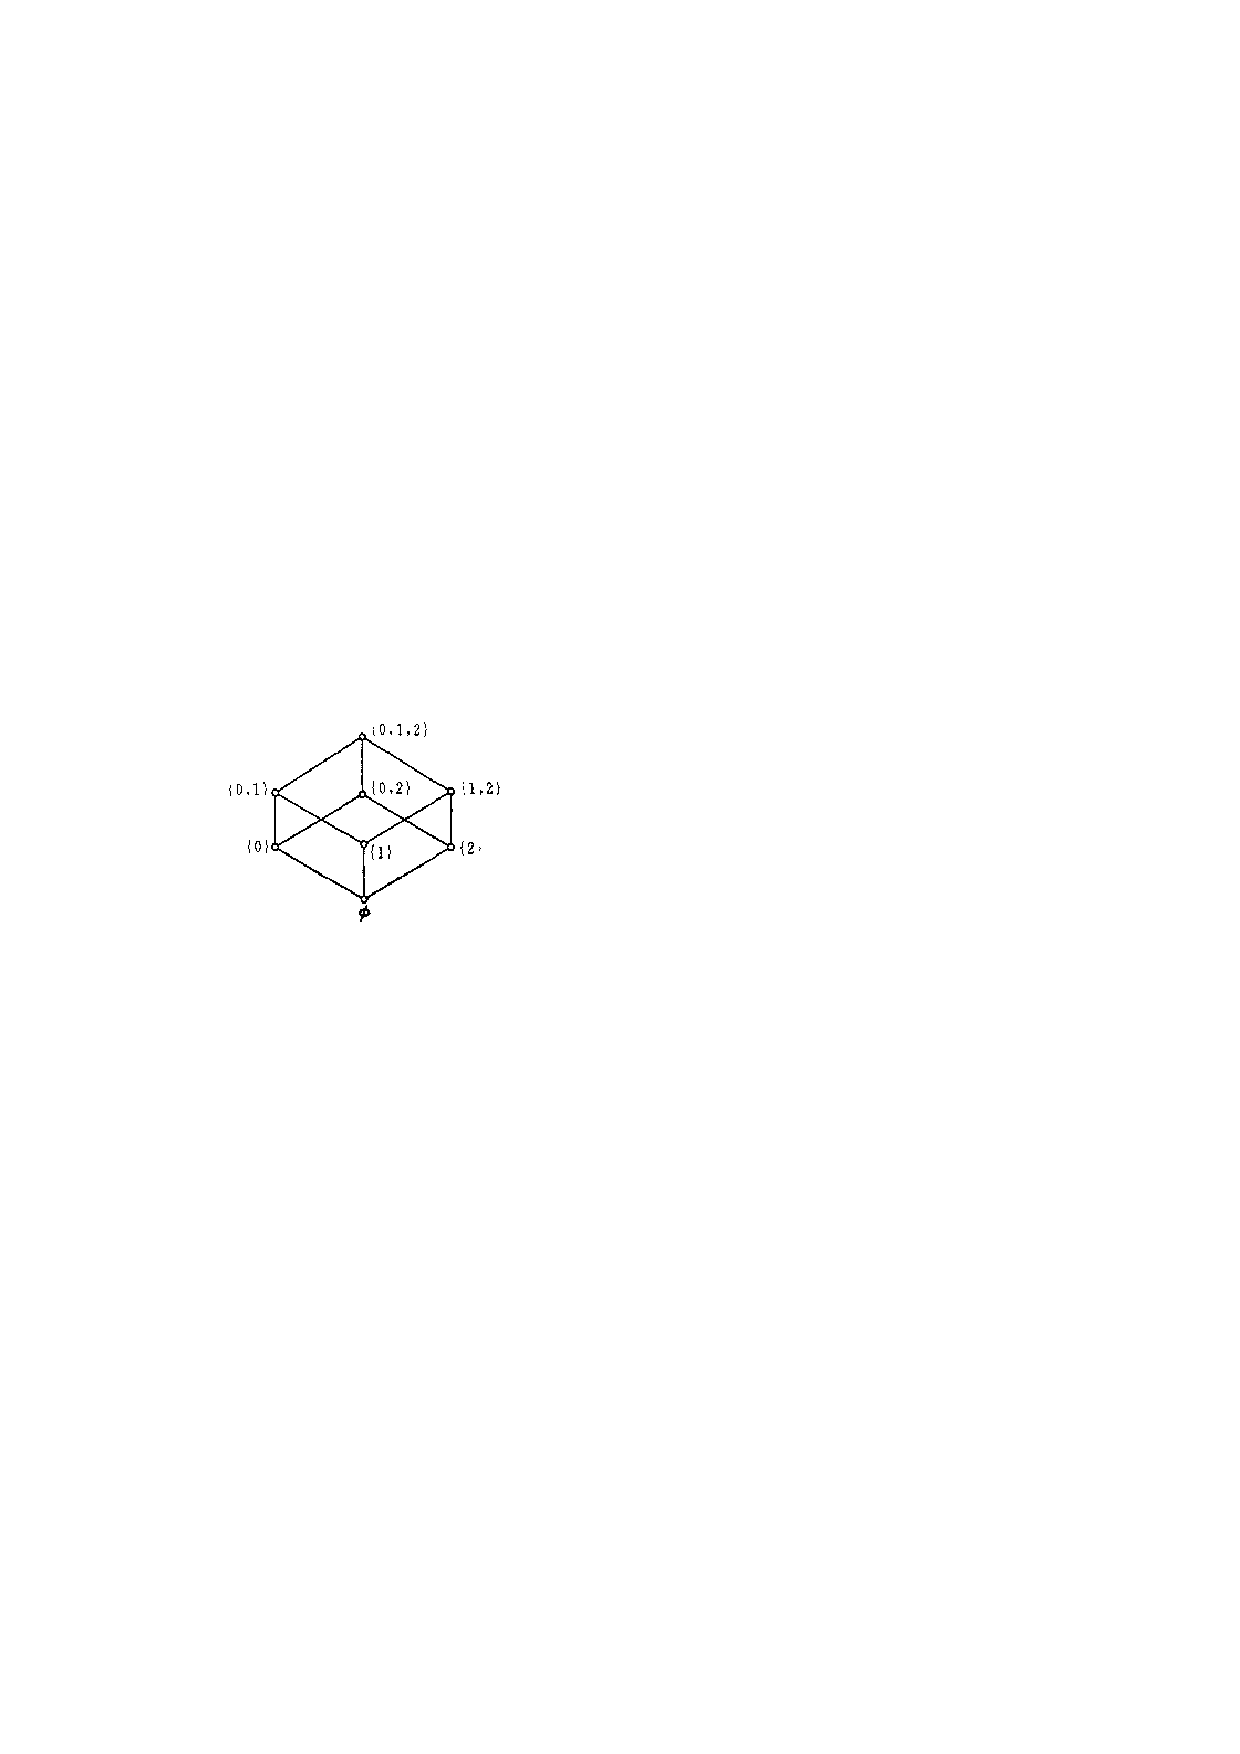
\includegraphics[width=0.6\linewidth]{graph-miji.pdf}
	 \caption{幂集图示法}
	\end{figure}
	\begin{figure}[!htp]
	 \centering
	 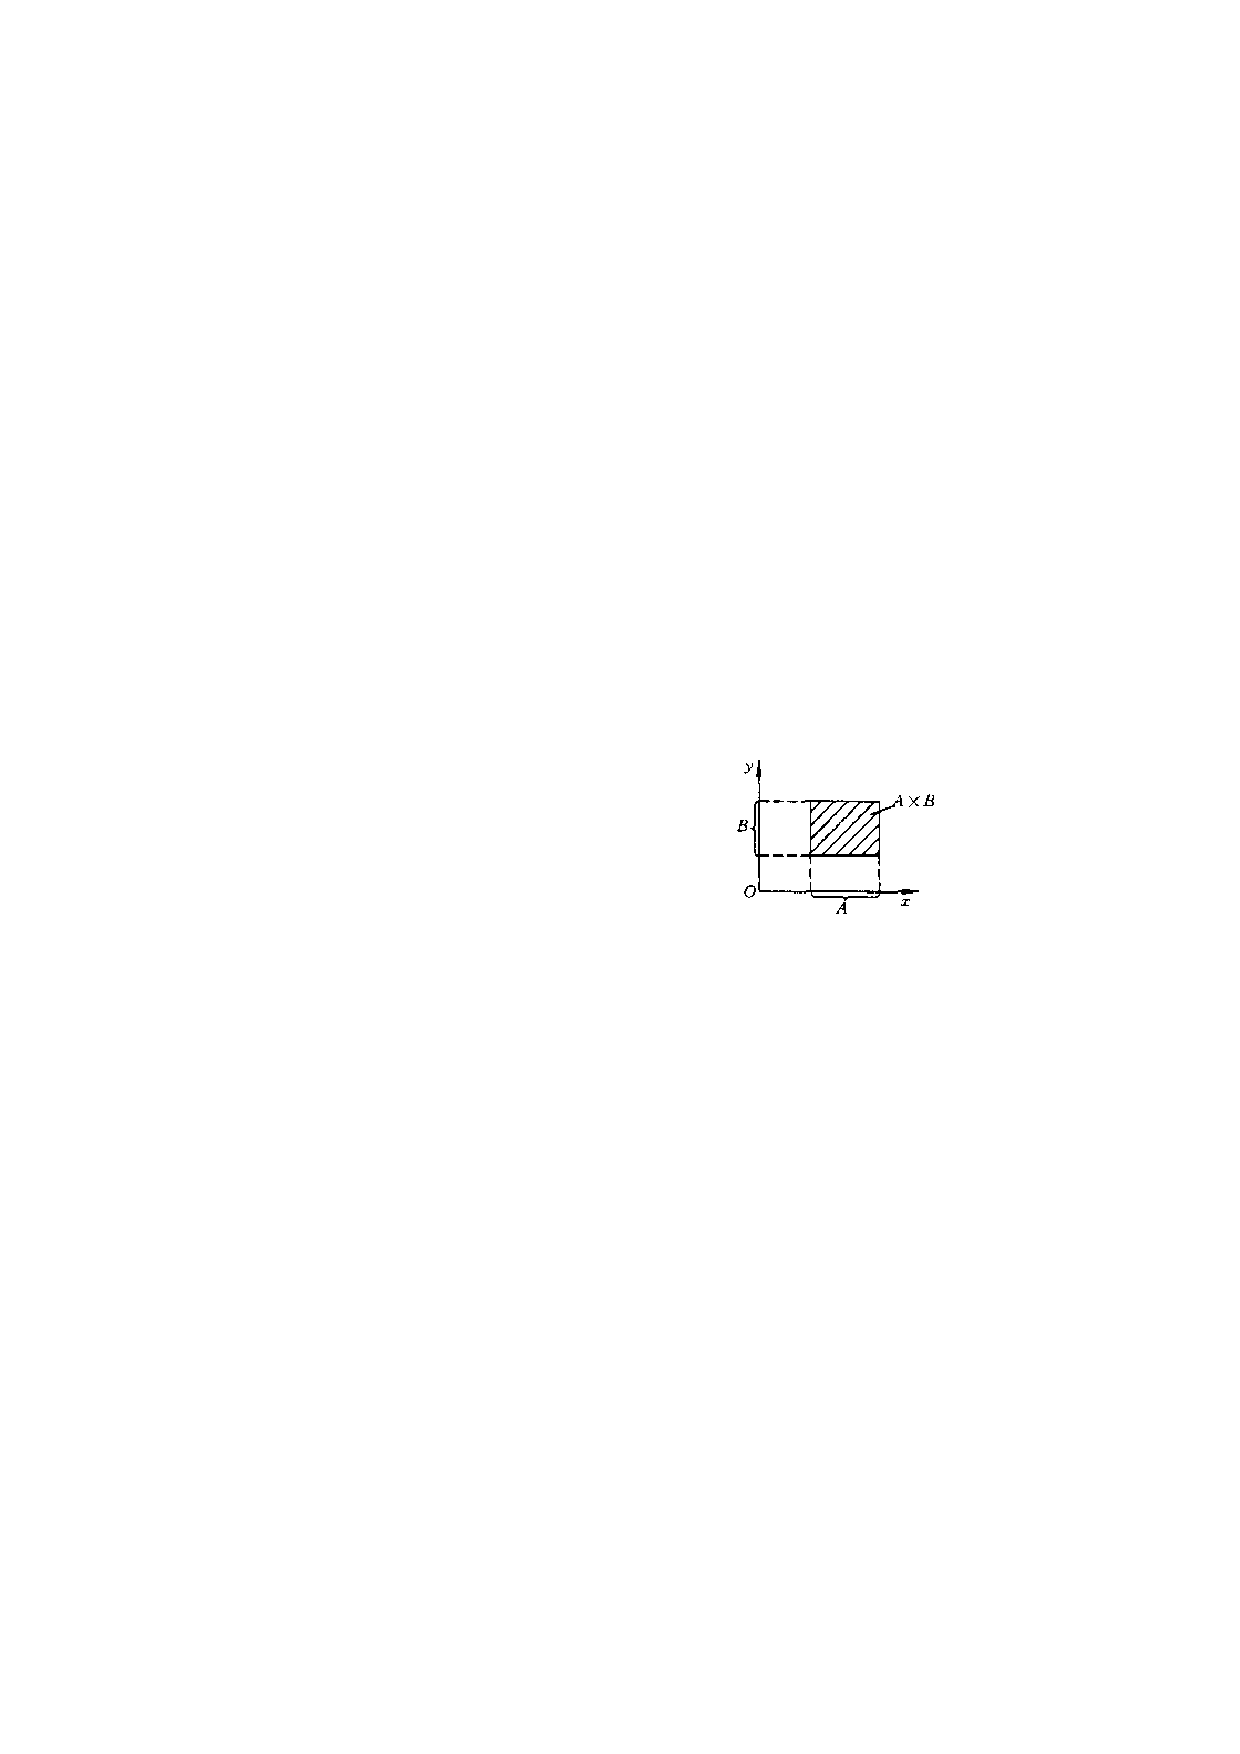
\includegraphics[width=0.6\linewidth]{graph-dikaer.pdf}
	 \caption{笛卡尔积图示法}
	\end{figure}
\end{enumerate}
\subsection{集合的运算性质} % (fold)
\label{sub:set_calculation}
\begin{enumerate}
	\item 交换律与结合律 $\cap, \cup$
	\item 分配率 $\cap$ 与 $\cup$ 互相
	\item 幂等律 $A\cup A = A \cap A = A$
	\item 吸收率 $A\cup(A\cap B) = A\cap (A\cup B) = A$
	\item 摩根率\\
	$A - (B\cup C) = (A-B)\cap (A-C)$\\
	$A - (B\cap C) = (A-B)\cup (A-C)$
	\item 同一律 $A\cup\emptyset = A\cap E = A$
	\item 零律 $A\cup E = E$, $A\cap\emptyset = \emptyset$
	\item 补余率 $A\cup -A = E$, $A\cap -A = \emptyset$
	\item 双补律 $-(-A) = A$
	\item 差集的性质
	\begin{itemize}
		\item $A-B = A-(A\cap B)$
		\item $A-B = A\cap -B$
		\item $A\cup (B-A) = A\cup A$
		\item $A\cap (B-C) = (A\cap B) - C$
	\end{itemize}
	\item 对称差的性质
	\begin{itemize}
		\item $A\oplus B = B\oplus A$
		\item $(A\oplus B)\oplus C = A\oplus (B\oplus C)$
		\item $A\cap(B\oplus C) = (A\cap B)\oplus (A\cap C)$
		\item $A\oplus \emptyset = A$, $A\oplus A = \emptyset$
		\item $A\oplus(A\oplus B) = B$
	\end{itemize}
\end{enumerate}
% subsection set_calculation (end)
\subsection{集合的关系性质} % (fold)
\label{sub:set_relation}
\begin{enumerate}
	\item 任意集合
	\begin{align*}
		&A\subseteq B \Rightarrow (A\cup C)\subseteq (B\cup C) \\
		&A\subseteq B \Rightarrow (A\cap C)\subseteq (B\cap C) \\
		&(A\subseteq B) \land (C\subseteq D) 
		\Rightarrow (A\cup C)\subseteq(B\cup D)  \\
		&(A\subseteq B) \land (C\subseteq D) 
		\Rightarrow (A\cap C)\subseteq(B\cap D)  \\
		&(A\subseteq B) \land (C\subseteq D) 
		\Rightarrow (A - C)\subseteq(B - D)  \\
		&C\subseteq D \Rightarrow (A - D) \subseteq (A - C)
	\end{align*}
	\item 幂集的性质
	\begin{align*}
		&A\subseteq B \Leftrightarrow P(A) \subseteq P(B) \\
		&A = B \Leftrightarrow P(A) = P(B) \\
		&P(A) \in P(B) \Leftrightarrow A \in B \\
		&P(A) \cap P(B) = P(A\cap B) \\
		&P(A)\cup P(B) \subseteq P(A\cup B) \\
		&P(A-B)\subseteq (P(A)-P(B))\cup\{\emptyset\}
	\end{align*}
	\item 广义交和广义并
	\begin{align*}
		&A\subseteq B \Rightarrow \bigcup A \subseteq \bigcup B\\
		&A\subseteq B \Rightarrow \bigcap B \subseteq \bigcap A\\
		&\bigcup(A\cup B) = (\bigcup A)\cup(\bigcup B) \\
		&\bigcup(A\cup B) = (\bigcup A)\cap(\bigcup B) \\
		&\bigcup(P(A)) = A
	\end{align*}
	\item 传递集合 $(\forall x)(\forall y)((x\in y\land y\in A)\to x\in A)$\\
	$\Leftrightarrow A\subseteq P(A)$ 
	$\Leftrightarrow P(A)$ 是传递集合 \\
	$\Rightarrow \bigcup A$ 是传递集合 $\Leftarrow$ $A$ 的元素都是传递集合 \\
	$\Rightarrow $ $A\neq \emptyset \to \bigcap A = \emptyset$ (由正则公理导出)\\
	$A$ 的元素都是传递集合, 则 $\cap A$ 是传递集合
	\item 笛卡尔积一般不满足交换律和结合律. 
	($A\times \emptyset = \emptyset\times A = \emptyset$)
	\item $x,y\in A \Rightarrow \langle x, y \rangle \in PP(A)\equiv P(P(A))$
	\item 笛卡尔积的性质
	\begin{align*}
		& A\times (B\cup C) = (A\times B)\cup (A\times C) \\
		& A\times (B\cap C) = (A\times B)\cap (A\times C) \\
		& (B \cup C)\times A = (B\times A)\cup (C\times A) \\
		& (B \cap C)\times A = (B\times A)\cap (C\times A) \\
		& A\subseteq B \Leftrightarrow A\times C\subseteq B\times C
		\Leftrightarrow C\times A \subseteq C\times B \\
		& A\times B \subseteq C\times D 
		\Leftrightarrow A\subseteq C\land B\subseteq D
	\end{align*}
\end{enumerate}
% subsection set_relation (end)
\subsection{有限集合的基数} % (fold)
\label{sub:limited_set_num}
\begin{enumerate}
	\item 有限集合基数 (cardinal number, potency) 记作
	$|A| = n$ 或 $\mathrm{card}(A) = n$. $|\emptyset | = 0$
	\item $|P(A)|=2^{|A|}$, $|A\times B|=|A|\cdot|B|$
	\item 对于集合 $A, B$
	\begin{align*}
		&|A\cup B| = |A| + |B| - |A\cap B| \le |A| + |B| \\
		&|A\cap B| \le \min (|A|, |B|) \\
		&|A-B| \ge |A|-|B| \\
		&|A\oplus B| = |A| + |B| - 2|A\cap B|
	\end{align*}
\end{enumerate}
% subsection limited_set_num (end)
\subsection{集合公理系统} % (fold)
\label{sub:set_axiom}
任一集合的所有元素都是集合, 其他对象用集合定义. 集合论公理系统的目的: 
\begin{itemize}
	\item 判定集合的存在性
	\item 构造所有合法集合 (合法性)
\end{itemize}
ZF (Zermelo-Frankel) 集合论公理系统: 
\footnote{其他还有 GB (Godel \& Bernays) 公理系统等.}
\begin{enumerate}
	\item 外延公理: 集合相等的条件\\
	$(\forall x)(\forall y)(x=y \leftrightarrow 
	(\forall z)(z\in x \leftrightarrow z\in y)$
	\item 空集存在公理: 定义空集 \\
	$(\exists x)(\forall y)(y\notin x)$ \\
	且由外延公理, 空集是唯一的, 记为 $y=\emptyset$
	\item 无序对集合存在公理*: \label{pair_exist}\\
	$(\forall x)(\forall y)(\exists z)(\forall u)
	(u\in z \leftrightarrow (u=x\lor u=y) )$
	\item 并集合存在公理: 集合的广义并的存在性\\
	$(\forall x)(\exists y)(\forall z)(z\in y \leftrightarrow 
	(\exists u)(z\in u \land u\in x))$
	\item 子集公理模式 (分离公理模式)*: \label{subset_form}\\
	$(\forall x)(\exists y)(\forall z)(z\in y 
	\leftrightarrow (z\in x \land P(z)))$\\
	谓词公式 $P(z)$ 任取 (公理模式), 
	交集, 差集, 广义交和笛卡儿积
	\footnote{$x\in A \land y\in B \Rightarrow\langle x, y \rangle \in PP(A\cup B)$}
	的存在性
	\begin{itemize}
		\item 不存在一切集合的集合: \\
		若存在这样的 $A$, 由子集公理, 令 $A_0 = \{x|x\in A\land x\notin x\}$, 
		即 $x\in A \Leftrightarrow x\in A\land x\neq x$. 令 $x = A_0$ 可得矛盾. 
		($\bigcap \emptyset$ 不存在)
	\end{itemize}
	\item 幂集合公理: 定义幂集 $y = P(x)$\\
	$(\forall x)(\exists y)(\forall z)(z\in y \leftrightarrow
	(\forall u)(u\in z \to u \in x))$
	\item 正则公理: (排除奇异集合)\\
	$(\forall x)(x\neq \emptyset \rightarrow 
	(\exists y)(y\in x\land (x\cap y = \emptyset)))$\\
	称 $y$ 为 $x$ 的极小元
	\begin{itemize}
		\item $(\forall A)(A\neq A)$
		\item $(\forall A_1)(\forall A_2)\lnot(A_1\in A_2 \land A_2 \in A_1)$
		\item 奇异集合 $A$ 定义: \\
		存在集合序列 $A_i (i\in\mathbb N)$, 使得 $A_i\in A \land A_{i+1}\in A_i$
		\item 满足正则公理等价于不是奇异集合
		\item $(\forall A)$ $A\neq\emptyset$ 是传递集合 
		$\rightarrow \emptyset\in A$
	\end{itemize}
	\item 无穷公理: 定义自然数集合 $x = \mathbb N$\\
	$(\exists x)(\emptyset\in x \land (\forall y)(y\in x \to 
	(y\cup \{y\})\in x))$
	\begin{itemize}
		\item 这个定义下 $m<n \Leftrightarrow m\subset n$
		\item 集合的三歧性: $(\forall x)(\forall y)((x\in A \land y\in A)
		\rightarrow (x\in y \lor x=y \lor y\in x))$. 自然数集合 $\mathbb N$ 
		与每个自然数 $n\in\mathbb N$ 都有三歧性
	\end{itemize}
	\item 替换公理模式: 子集公理模式的二元推广\\
	$(\forall x)(\exists ! y) P(x,y) \to (\forall t)(\exists s)\tilde P(s, t)$ \\
	其中$(\exists ! y) P(x,y)$ 表示\\
	$(\exists y) (P(x,y)\land (\forall z)(P(x,z)\to z=y))$\\
	$\tilde P(s, t)$ 表示 \\
	$ (\forall u)(u\in s \leftrightarrow (\exists z)(z \in t \land P(z, u))$
	\begin{itemize}
		\item 根据空集定理和幂集定理, $PP(\emptyset)$ 是集合. 令 $P(\emptyset,x)
		= P(\{\emptyset\}, y) = T$ 得到 (\ref{pair_exist}) 无序对集合存在
		\item 令 $P(x,y) = p(x)\land (x=y)$ 即为 (\ref{subset_form}) 子集公理模式
	\end{itemize}
	\item 选择公理: \\
	$(\forall x) (R(x) \to (\exists u) S(x,u))$\\
	其中 $R(x)$ 表示\\
	$(\forall y)\big((y\in x \to y \neq \emptyset)\land (\forall y)(\forall z)
	((y\in x\land z\in x \land y\neq z)\to (y\cap z=\emptyset))\big)$\\
	$S(x,u)$ 表示\\
	$(\forall y)(y\in x \to (\exists !t)(t\in y \land t \in u)$.\\
	\begin{itemize}
		\item 等价于: 对于任意关系存在子集为函数, 且定义域相等
	\end{itemize}
\end{enumerate}
* 其中 (\ref{pair_exist}) 无序对集合存在与 (\ref{subset_form}) 
子集公理模式可由其他公理导出
% subsection set_axiom (end)
\subsection{关系的定义} % (fold)
\label{sub:relationship}
\begin{enumerate}
	\item 二元关系: 有序对的集合或者空集, 记作 $R$. $\langle x, y \rangle \in R$
	记作 $xRy$
	\item $A\times B$ 的子集定义 $A$ 到 $B$ 的二元关系; 
	特别的 $A\times A$ 的子集定义 $A$ 上的二元关系
	\item $n$ 元关系: $A_1\times \cdots \times A_n$ 的子集
	\item 特殊的二元关系: 
	\begin{itemize}
		\item 恒等关系 \\
		$I_A = \{\langle x, x \rangle | x\in A\}$
		\item 全关系/全域关系 \\
		$E_A = \{\langle x, y \rangle | x\in A\land y\in A\}$
		\item 空关系 $\emptyset$
	\end{itemize}
	\item 定义域 ($\dom$), 值域 ($\ran$) 和域 ($\fld$): 
	\begin{itemize}
		\item $\dom(R) = \{x|(\exists y)(\langle x, y \rangle \in R)\}$
		\item $\ran(R) = \{y|(\exists x)(\langle x, y \rangle \in R)\}$
		\item $\fld(R) = \dom(R)\cup\ran(R) = \left(\bigcup\bigcup R\right)$
	\end{itemize}
	\item 关系的逆 $R^{-1}$\\
	$R^{-1} = \{ \langle x, y \rangle | \langle y, x \rangle \in R \}$
	\item 关系的合成 $S\circ R$\\
	$S\circ R = \{ \langle x, z \rangle | (\exists y) 
	( \langle x, y \rangle \in R \land \langle y, z \rangle \in S)\}$
	\begin{itemize}
		\item $R_1\circ (R_2\cup R_3) = R_1\circ R_2 \cup R_1 \circ R_3$
		\item $R_1\circ (R_2\cap R_3) \subseteq R_1\circ R_2 \cap R_1 \circ R_3$
		\item $(R_1 \cup R_2)\circ R_3 = R_1\circ R_3 \cup R_2 \circ R_3$
		\item $(R_1 \cap R_2)\circ R_3 \subseteq R_1\circ R_3 \cap R_2\circ R_3$
	\end{itemize}
	\item 关系在集合上的限制 $R\upharpoonright A$ \\
	$R \upharpoonright A = \{ \langle x, y \rangle | \langle x, y \rangle \in R
	\land x \in A\}$
	\item 集合在关系下的象 $R[A]$ \\
	$R[A] = \{y|(\exists x)(x\in A \land \langle x, y \rangle \in R\}$
	\begin{itemize}
		\item $R[\bigcup A] = \bigcup\{R[B]|B\in A\}$
		\item $R[\bigcap A] \subseteq \bigcap\{R[B]|B\in A\}$
		\item $R[A] - R[B] \subseteq R[A-B]$
	\end{itemize}
	\item 关系矩阵 $\bm{M}(R)$: 对于 $R\subseteq X\times Y$, 
	$\bm{M}(R) = (r_{ij})_{|X|\times|Y|}$, 其中
	$$
	r_{ij} = \begin{cases}
		1, & \langle x_i, y_j \rangle \in R \\
		0, & \langle x_i, y_j \rangle \notin R
	\end{cases}
	$$
	\begin{itemize}
		\item 布尔数域上 $\bm M(S\circ R) = \bm M (R) \bm M(S)$
	\end{itemize}
	\item 关系图 $G(R) = \langle V, E \rangle$ (有向图): 
	对于 $R\subseteq X\times Y$, 
	$V = X\cup Y$, $E = \{e_{ij}|\langle x_i, y_j\rangle\in R\}$
\end{enumerate}
% subsection relationship (end)
\subsection{关系的性质} % (fold)
\label{sub:chara_of_relation}
$R$ 在 $A$ 上: 
\begin{enumerate}
	\item 自反: $(\forall x)(x\in A \to xRx)$
	\begin{itemize}
		\item $R_1, R_2$ 是自反的, 
		则 $R_1^{-1}, R_1\cap R_2, R_1\cup R_2$ 也是自反的
	\end{itemize}
	\item 非自反: $(\forall x)(x\in A \to x\not\negthickspace{R}x)$
	\item 对称: $(\forall x)(\forall y)((x\in A\land y \in A \land x R y)
	\to yRx)$
	\begin{itemize}
		\item $R_1, R_2$ 是对称的, 
		则 $R_1^{-1}, R_1\cap R_2, R_1\cup R_2$ 也是对称的
		\item $R$ 是对称的, 则 $R^{-1} = R$
	\end{itemize}
	\item 反对称: $(\forall x)(\forall y)(
	(x\in A\land y \in A \land xRy \land yRx)\to x=y)$
	\begin{itemize}
		\item $R_1, R_2$ 是反对称的, 
		则 $R_1^{-1}, R_1\cap R_2$ 也是反对称的
		\item $R$ 是反对称的, 则 $R\cap R^{-1} = I_A$
	\end{itemize}
	\item 传递: $(\forall x)(\forall y)(\forall z)
	((x\in A\land y\in A \land z\in A\land xRy\land yRz)\to xRz)$
	\begin{itemize}
		\item $R_1, R_2$ 是传递的, 
		则 $R_1^{-1}, R_1\cap R_2$ 也是传递的
	\end{itemize}
\begin{table}[!htp]
 \centering
 \caption{关系的特征}
 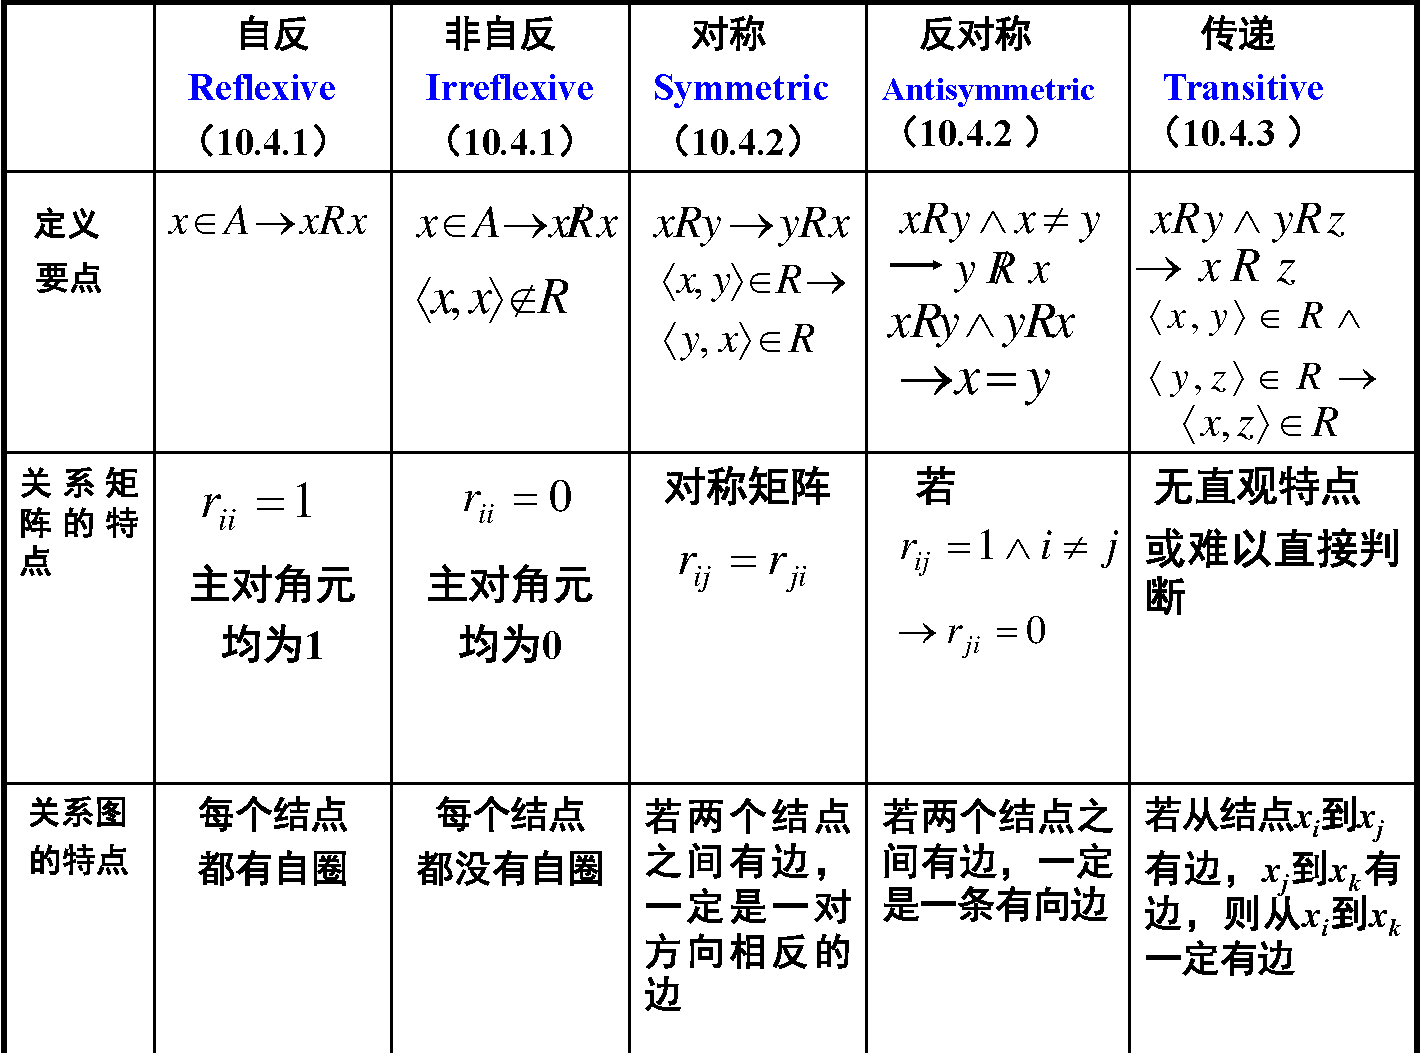
\includegraphics[width=\linewidth]{relationship.pdf}
 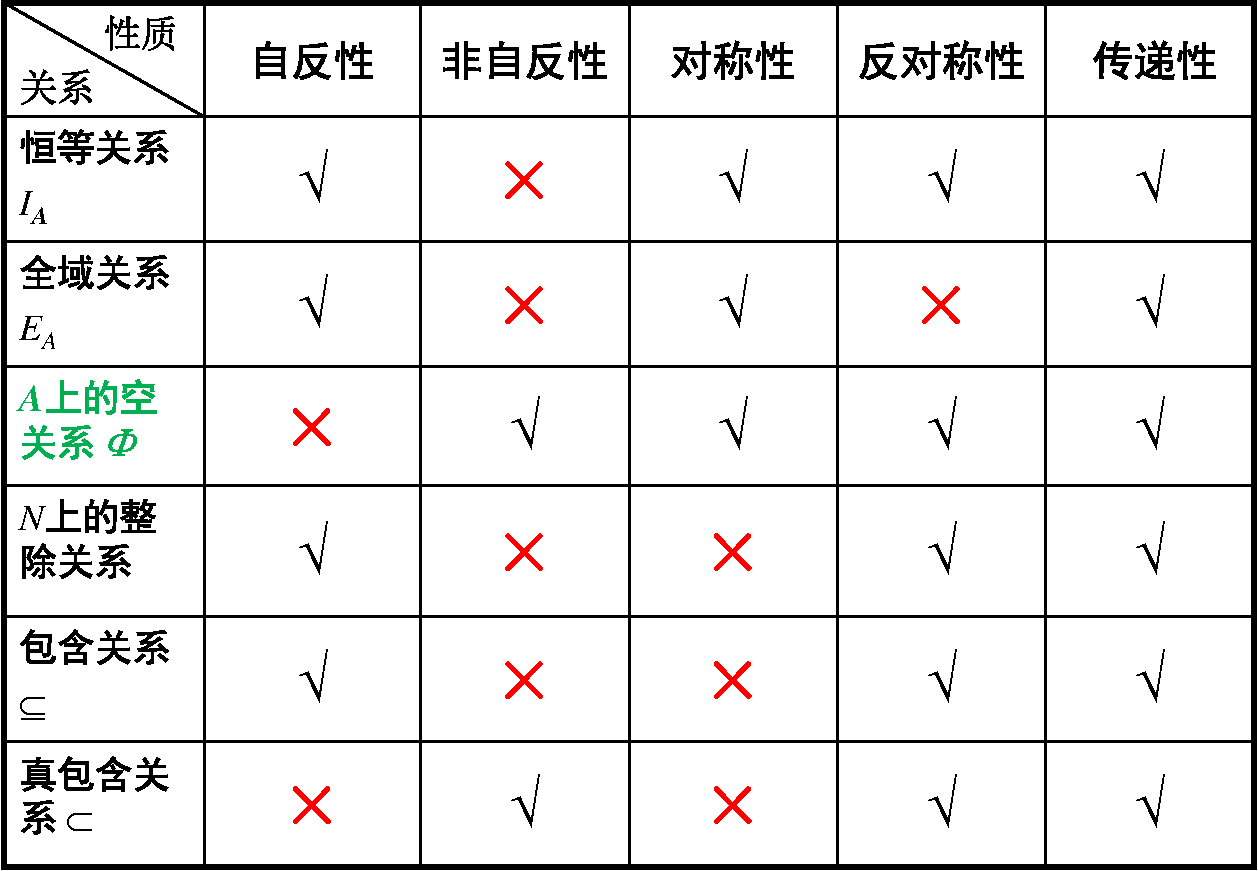
\includegraphics[width=\linewidth]{relationship-egs.pdf}
\end{table}
\begin{table}[!htp]
 \centering
 \caption{关系的运算特征}
 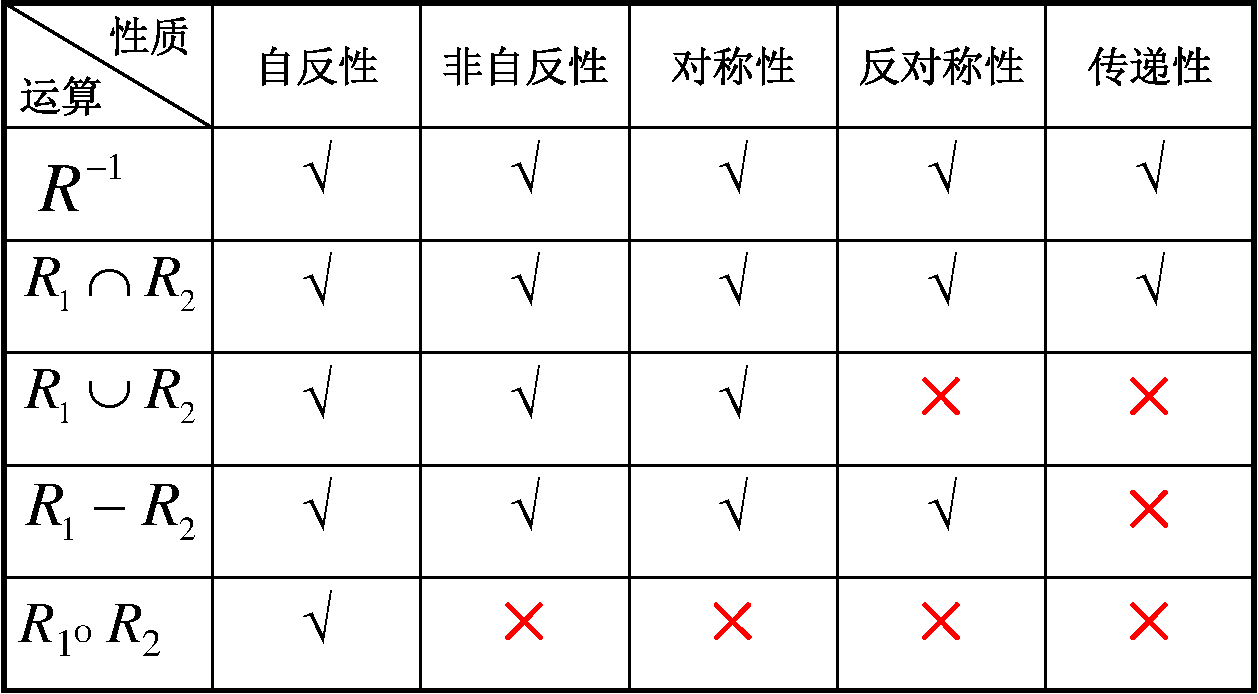
\includegraphics[width=\linewidth]{relationship-cal.pdf}
\end{table}
\end{enumerate}
% subsection chara_of_relation (end)
\subsection{关系的闭包} % (fold)
\label{sub:closure}
\begin{enumerate}
	\item 递归推广关系合成到 $R^n$
	\item 定理: 
	\begin{itemize}
		\item 有限集合 $A$ 上的关系 $R$, 存在自然数 $s \neq t$ 使 $R^s = R^t$ 
		(鸽巢原理)
		\item $p = |s-t|$, $B = \{R^0 = I_A, R^1, \cdots, R^{t-1}\}$, 则
		$(\forall q)(q\in\mathbb N \to R^q\in B\}$
	\end{itemize}
	\item 闭包: 对于 $A\neq\emptyset$ 上的关系 $R$, 若 $R'$ 满足
	\begin{enumerate}
		\item $R'$ 是自反的 (对称的, 传递的)
		\item $R\subseteq R'$
		\item $(\forall R'')$ $R''$ 是 $A$ 上自反的 (对称的, 传递的) 关系, 
		$R\subseteq R'' \to R'\subseteq R''$
	\end{enumerate}
	则称 $R'$ 为关系 $R$ 的自反 (对称, 传递) 闭包, 记作 $r(R)$ ($s(R)$, $t(R)$)
	\item 闭包的性质
	\begin{itemize}
		\item $R$ 是自反的 (对称的, 传递的) 等价于其闭包是自身
		\item $R_1 \subseteq R_2 \rightarrow x(R_1)\subseteq x(R_x)$. 
		($x = r,s,t$)
		\item $r(R_1)\cup r(R_2) = r(R_1\cup R_2)$
		\item $s(R_1)\cup s(R_2) = s(R_1\cup R_2)$
		\item $t(R_1)\cup t(R_2) \subseteq t(R_1\cup R_2)$
		\item $R$ 是自反的, 则 $s(R)$ 和 $t(R)$ 是自反的
		\item $R$ 是对称的, 则 $r(R)$ 和 $t(R)$ 是对称的
		\item $R$ 是传递的, 则 $r(R)$ 是传递的
		\item $rs(R) = sr(R)$
		\item $rt(R) = tr(R)$
		\item $st(R)\subseteq ts(R)$
	\end{itemize}
	\item 闭包的构造
	\begin{itemize}
		\item $r(R) = R\cup R^0$
		\item $s(R) = R\cup R^{-1}$
		\item $t(R) = R\cup R^2\cup R^3\cup\cdots$
	\end{itemize}
	特别的, 存在 $k\le n$ 使 $t(R) =  R\cup\cdots\cup R^k$
	\item 传递闭包构造的 Warshall 算法
	\begin{lstlisting}[mathescape, caption=Warshall 算法]
for i=1 to n, j=1 to n, k=1 to n
	$r_{jk} = r_{jk}\lor (r_{ji}\land r_{ik})$
	\end{lstlisting}
\end{enumerate}
% subsection closure (end)
\subsection{等价关系和划分} % (fold)
\label{sub:equivalent}
\begin{enumerate}
	\item 等价关系: 自反, 对称和传递的关系
	\item 等价类 $[x]_R = \{y|y\in A \land x R y\}$, 或记作 $[x], \overline x$
	\item 全部等价类的集合: 商集, 记作 $A/R$
	\item 划分 $\pi$ (不多, 非空, 不漏, 不重): 
	\begin{enumerate}
		\item $(\forall x)(x\in \pi \to x\subseteq A)$
		\item $\emptyset \notin \pi$
		\item $\bigcup \pi = A$
		\item $(\forall x)(\forall y)((x\in \pi \land y\in \pi \land x\neq y)
		\to x\cap y - \emptyset)$
	\end{enumerate}
	\item 等价类是一个划分
	\item 等价关系诱导划分 $\pi_R$; 划分诱导等价关系 $R_\pi$. 
	\item $\pi = \pi_R \leftrightarrow R = R_\pi$
\end{enumerate}
% subsection equivalent (end)
\subsection{相容关系和覆盖} % (fold)
\label{sub:compatibility}
\begin{enumerate}
	\item 相容关系: 自反和对称的关系
	\item 相容类 $C = \{x|x\in A\land (\forall y)(y \in C \to x R y)\}$
	\item 最大相容类 $C_R$ 不是任何相容类的真子集\\
	$(\forall x)(x\in A - C_R \to (\exists y)(y\in C_R \land 
	x\not\not\negthickspace{R} y))$
	\item 非空有限集合上的任何相容类存在最大相容类超集
	\item 覆盖 $\Omega$ (不多, 非空, 不漏):
	\begin{enumerate}
		\item $(\forall x)(x\in \Omega \to x\subseteq A)$
		\item $\emptyset \notin \Omega$
		\item $\bigcup \Omega = A$
	\end{enumerate}
	\item 完全覆盖: 最大相容类的集合 $C_R(A)$. 完全覆盖是唯一的
\end{enumerate}
% subsection compatibility (end)
\subsection{偏序关系与上下界} % (fold)
\label{sub:partial_ordering}
\begin{enumerate}
	\item 偏序关系: 自反, 反对称, 传递的关系, 记作 $\le$
	\item 拟序关系: 非自反, 传递的关系, 记作 $<$
	\begin{itemize}
		\item 拟序关系是反对称的
	\end{itemize}
	\item 对于拟序关系 $R$, $R\cup R^0$ 是偏序关系
	\item 对于偏序关系 $R$, $R - R^0$ 是拟序关系
	\item $A$ 和 $A$ 上关系 $R$ 称为结构 $\langle A, R \rangle$. 
	偏序结构或称偏序集
	\item 盖住: 对于偏序集 $\langle A, \le \rangle$, 对于 $x, y\in A$ 
	且 $x\le y \land x\neq y$, 如果 $\lnot(\exists z)(x\le z \le y)$, 
	则称 $y$ 盖住 $x$
	\item $A$ 上的盖住关系 $\mathrm{cov}A = \{\langle x, y \rangle$ 是唯一的
	\item 哈斯 (Hasse) 图
	\begin{enumerate}
		\item 每个顶点代表一个元素
		\item $x\le y$ 且 $x\neq y$ 则 $y$ 在 $x$ 的上方
		\item $\langle x, y \rangle \in \mathrm{cov}A$ 则连无向边
	\end{enumerate}
	\item 对于偏序关系 $\langle A, \le \rangle$, 且 $B\subseteq A$
	\begin{enumerate}
		\item $(\exists y)(y\in B \land (\forall x)(x\in B \to y\le x))$: 
		$y$ 为 $B$ 的最小元
		\item $(\exists y)(y\in B \land (\forall x)(x\in B \to x\le y))$: 
		$y$ 为 $B$ 的最大元
		\item $(\exists y)(y\in B \land (\forall x)((x\in B\land x\le y) \to x=y))$: 
		$y$ 为 $B$ 的极小元
		\item $(\exists y)(y\in B \land (\forall x)((x\in B\land y\le x) \to x=y))$: 
		$y$ 为 $B$ 的极大元
		\item 最小 (大) 元不一定存在, 存在必定唯一; 
		极小 (大) 元一定存在, 不一定唯一
		\item $(\exists y)(y\in A \land (\forall x)(x\in B \to x\le y))$: 
		$y$ 为 $B$ 的上界
		\item 上确界 (最小上界): 上界集合的最小元
		\item $(\exists y)(y\in A \land (\forall x)(x\in B \to y\le x))$: 
		$y$ 为 $B$ 的下界
		\item 下确界 (最小下界): 下界集合的最大元
		\item 上下界不一定存在, 不一定唯一; 上下确界不一定存在, 存在一定唯一
	\end{enumerate}
\end{enumerate}
\subsubsection{全系关系} % (fold)
\label{ssub:full_ordering}
\begin{enumerate}
	\item 可比的: $x\le y \lor y\le x$
	\item 全序关系 (线序关系): 任意两个元素可比. 全序集
	\item  对于偏序关系 $\langle A, \le \rangle$, 且 $B\subseteq A$
	\begin{enumerate}
		\item 链 $B$: 元素都可比. 链的长度
		\item 反链 $B$: 元素都不可比. 反链的长度
	\end{enumerate}
	\item $\langle A, \le \rangle$ 中最长链的长度 $n$, 则将元素分成不相交的反链, 
	反链的个数至少是 $n$. \\
	极大元的集合是一条反链. 据此做数学归纳可证明
\end{enumerate}
% subsubsection full_ordering (end)
\subsubsection{良序关系} % (fold)
\label{ssub:well_ordering}
\begin{enumerate}
	\item 良序关系: 任何非空子集都有最小元. 良序集
	\item 良序集一定是全序集. 取二元子集可证
	\item 有限全序集一定是良序集
	\item 良序化: 定义良序关系
	\item 任意集合都可以良序化 (由选择公理证明)
\end{enumerate}
% subsubsection well_ordering (end)
% subsection partial_ordering (end)
% section set_theory (end)
\end{document}
一二四五九十
十一十二的部分